\documentclass[eng]{JuLIET-class}

% Publication Title
\title{Judul Makalah}

% Authors
\author[1]{Penulis A*}
\author[2]{Penulis B}
\author[3]{Penulis C}

% Author Affiliations
\affil[1]{Nama Departemen, Nama Afiliasi 1; penulis b@email.com}
\affil[2]{Nama Departemen, Nama Afiliasi 1; penulis b@email.com}
\affil[*]{Korespondensi: penulis a@email.com}

% Surname of the first author of the manuscript
\firstauthor{SurnameA, SurnameB, and SurnameC}

%Contact Author Information
\inputpublishnum{E-ISSN: 2746-2536}% Name and surname of   

% Publication data (will be defined in the edition)
\thisvolume{XX}
\thisnumber{XX}
\thismonth{Month}
\thisyear{20XX}
\receptiondate{dd/mm/aaaa}
\acceptancedate{dd/mm/aaaa}
\publicationdate{dd/mm/aaaa}

% Place your particular definitions here
\newcommand{\vect}[1]{\mathbf{#1}}  % vectors
% Insert here the abstract in Eng
\abstract{
	One paragraph contains a maximum of 250 words. The abstract must represent the purpose of the article and must not contain results that are not presented and substantiated in the main text. Authors are advised to use the following structured abstract style: (1) Background: Describe the general problem in your field and the specific problem you want to solve; (2) Method: Briefly describe the method used to solve the problem; (3) Results: Summarizing the main findings of the article; (4) Conclusion: Shows the main conclusions or interpretations and implications of the article.
}

% Insert here the keywords of your work in English language
\keywords{keyword 1, keyword 2, keyword 3 (at most 5)}

% Insert here the abstract in Indo
\abstrak{Satu paragraf berisi maksimal 250 kata. Abstrak harus merepresentasikan tujuan dari artikel dan tidak boleh mengandung hasil yang tidak disajikan dan dibuktikan dalam naskah utama. Dianjurkan kepada penulis untuk menggunakan gaya abstrak terstruktur berikut: (1) Latar Belakang: Menjelaskan problem umum di bidang Anda dan problem khusus yang ingin diselesaikan; (2) Metode: Menjelaskan secara singkat metode yang digunakan untuk menyelesaikan permasalahan; (3) Hasil: Merangkum temuan utama dari artikel; (4) Simpulan: Menunjukkan simpulan atau interpretasi utama serta implikasi dari artikel.}

% Insert here the keywords of your work in English language
\katakunci{kata kunci 1, kata kunci 2, kata kunci 3 (maksimal 5)}

% Start document
\begin{document}
	
	\maketitle
	\thispagestyle{fancy}
	
	\section{\centering {PENDAHULUAN \textit{(Heading1)}}}
	Artikel ilmiah yang diterbitkan pada jurnal ini terdiri atas paling tidak lima bab, yaitu Pendahuluan, Dasar Teori, Metodologi, Hasil dan Pembahasan, dan Simpulan. Isi tiap-tiap bab akan dijelaskan pada template ini.
	Pendahuluan secara singkat berisi posisi studi dalam konteks bidang ilmu yang luas kemudian menuju pembahasan yang lebih khusus. Bagian ini harus mendefinisikan tujuan penelitian dan signifikansinya. Pustaka-pustaka yang memuat kondisi bidang penelitian terkini harus ditinjau dan dikutip. Jelaskan secara singkat tujuan utama penelitian dan tunjukkan kontribusi serta kebaruan utama dari artikel ini. Harap penulisan pendahuluan diupayakan memiliki aliran informasi yang dapat dipahami oleh individu di luar bidang penelitian Anda.
	
	Rujukan menggunakan style IEEE. Referensi harus diberi nomor sesuai urutan kemunculannya dan ditunjukkan dengan angka dalam tanda kurung siku—misalnya, \cite{NACA460} atau \cite{WangEtAl2015}, atau \cite{ArslanHansen1996,Indura2010,Krause2014}. Jika ingin merujuk, rujuk hanya ke nomor referensi, seperti “pada \cite{Mitchell2001}”, jangan gunakan “Ref. \cite{Mitchell2001}" atau "referensi \cite{Mitchell2001}" kecuali di awal kalimat, yaitu menggunakan "Referensi \cite{Mitchell2001} adalah yang pertama ...". 
	
	Sangat direkomendasikan untuk menggunakan Mendeley (\url{www.mendeley.com}) untuk pengorganisasian sumber pustaka. Lihat bagian akhir dokumen template ini untuk melihat rincian tentang referensi.
	
	
	\section{\centering{METODOLOGI}}    
	Metodologi berisi langkah-langkah dalam penelitian, metode yang digunakan, serta alasan menggunakan Langkah dan metode tersebut. Bagian ini  harus dijelaskan dengan detail sehingga memungkinkan orang lain untuk meniru dan meneruskan penelitian yang dipublikasikan.	
	
	
	\section{\centering{HASIL DAN PEMBAHASAN}}
	Hasil harus jelas dan ringkas. Bagian pembahasan harus menekankan pentingnya hasil pekerjaan. Penulis dapat menambahkan gambar dan tabel untuk menyampaikan hasil penelitian dan untuk mendukung pembahasan. Bab ini dapat memiliki subbab dengan format penomoran sebagai berikut:
	
	\subsection{Gambar dan Tabel (Heading 2)}
	Semua gambar dan tabel harus dikutip dalam teks utama seperti: “Pada Gambar 1 diilustrasikan…”, “Data disajikan pada Tabel 1”, dll. Gambar dan tabel diletakkan sedekat mungkin dengan paragraf yang merujuknya. Gambar 1 dan Tabel 1 menunjukkan contoh gambar dan tabel serta penulisan caption.
	\begin{enumerate}[wide, labelwidth=!, labelindent=0pt]
		\item [1)] Gambar \textit{(Heading 3)}: Gambar dapat ditampilkan dengan lebar maksimal 8 cm. Apabila gambar yang hendak ditampilkan lebih lebar, naskah dapat diatur menjadi satu kolom hanya pada gambar tersebut dan gambar diletakkan di paling atas atau paling bawah suatu halaman. Caption gambar diletakkan di bawah gambar dengan center alignment.
		\item [2)] \textit{Tabel: Header} tabel dicetak menggunakan huruf tebal dengan garis tebal hanya di atas header, di bawah header, dan di bawah tabel. Apabila tabel yang ditampilkan lebih lebar dari lebar kolom halaman, naskah dapat diatur menjadi satu kolom hanya pada tabel tersebut dan tabel diletakkan di paling atas atau paling bawah halaman. Caption tabel diletakkan di atas tabel dengan center alignment.
	\end{enumerate}
	\begin{figure}[H]
		\centering
		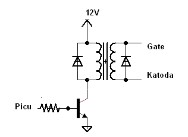
\includegraphics[scale=1]{Gambar/Gambar1.jpg}
		\caption{Skema rangkaian yang digunakan pada penelitian}
		\label{gambar_rangkaian}
	\end{figure}
	
	\begin{table}[H]
		\centering
		\caption{Hasil pengukuran besaran listrik}
		\begin{tabular}{@{}cccc@{}}
			\toprule
			Waktu & Tegangan (V) & Arus (A) & Impedansi ($\Omega$) \\ \midrule
			12:04 & 220 & 10 & 22 \\
			13:04 & 219 & 10 & 21,9 \\
			14:04 & 222 & 10 & 22,2 \\
			15:04 & 221 & 10 & 22,1 \\
			16:04 & 218 & 10 & 21,8 \\ \bottomrule
		\end{tabular}
	\end{table}
	\subsection{Persamaan}
	Seluruh persamaan menggunakan center alignment dan diikuti dengan nomor urut persamaan yang diletakkan di dalam tanda kurung. Contoh persamaan ditunjukkan oleh persamaan (1). Untuk merujuk persamaan dalam paragraf, gunakan “(1)”, bukan “Persamaan (1)” atau “persamaan (1)”, kecuali di awal kalimat, maka menggunakan “Persamaan (1) adalah . . .”.
	
	\begin{equation}
		V = L\frac{di}{dt}
	\end{equation}
	
	\subsection{Poin-Poin}
	Item-item juga dapat disajikan dalam bentuk poin-poin. Bulleting menggunakan titik berwarna hitam, seperti contoh pada paragraf selanjutnya.
	
	Beberapa jenis dokumen dalam referensi yang ditampilkan dalam bab Daftar Pustaka meliputi:
	
	\begin{itemize}
		\item Contoh buku [1]
		\item Contoh seri buku [2]
		\item Contoh artikel jurnal [3]
		\item Contoh makalah seminar [4]
		\item Contoh paten [5]
		\item Contoh dokumen/artikel pada website [6]
		\item Contoh dokumen laporan [7]
		\item Contoh tesis dan disertasi [8]
		
	\end{itemize}
	
	\section{\centering{SIMPULAN}}
	Bab simpulan berisi rangkuman dari permasalahan penelitian serta solusi yang ditawarkan untuk mengatasi permasalahan tersebut. Ditambah lagi, bab ini juga dapat memuat implikasi umum dari penelitian. Dengan menggunakan template ini, diharapkan naskah ilmiah yang dikirimkan akan memiliki format yang seragam dan mudah diikuti. Yang terakhir, halaman terakhir diupayakan memiliki panjang kolom yang sama.
	
	\section{\centering{UCAPAN TERIMAKASIH}}
	Ucapan terima kasih diberikan kepada pihak-pihak yang mendukung terlaksananya penelitian dan individu yang berkontribusi dalam penulisan naskah, tetapi tidak disebutkan sebagai penulis.
	
	% Include references
	\renewcommand\refname{\centering DAFTAR PUSTAKA}
	\bibliography{References.bib}

\end{document}